\section{Microcontroller}

Our microcontroller of choice, the Raspberry Pi 2 Model B, is a preferrable choice for embedded robotic systems. One of the deciding factors was the GPIO capabilities on the controller and the interface that it has to offer. It also features a powerful 900MHz quad-core ARM Cortex-A7 CPU and 1 GB of RAM. Because it has an ARMv7 processor, it can run the full range of ARM GNU/Linux distributions.\cite{raspispecs}

\begin{figure}[H]
	\centering
	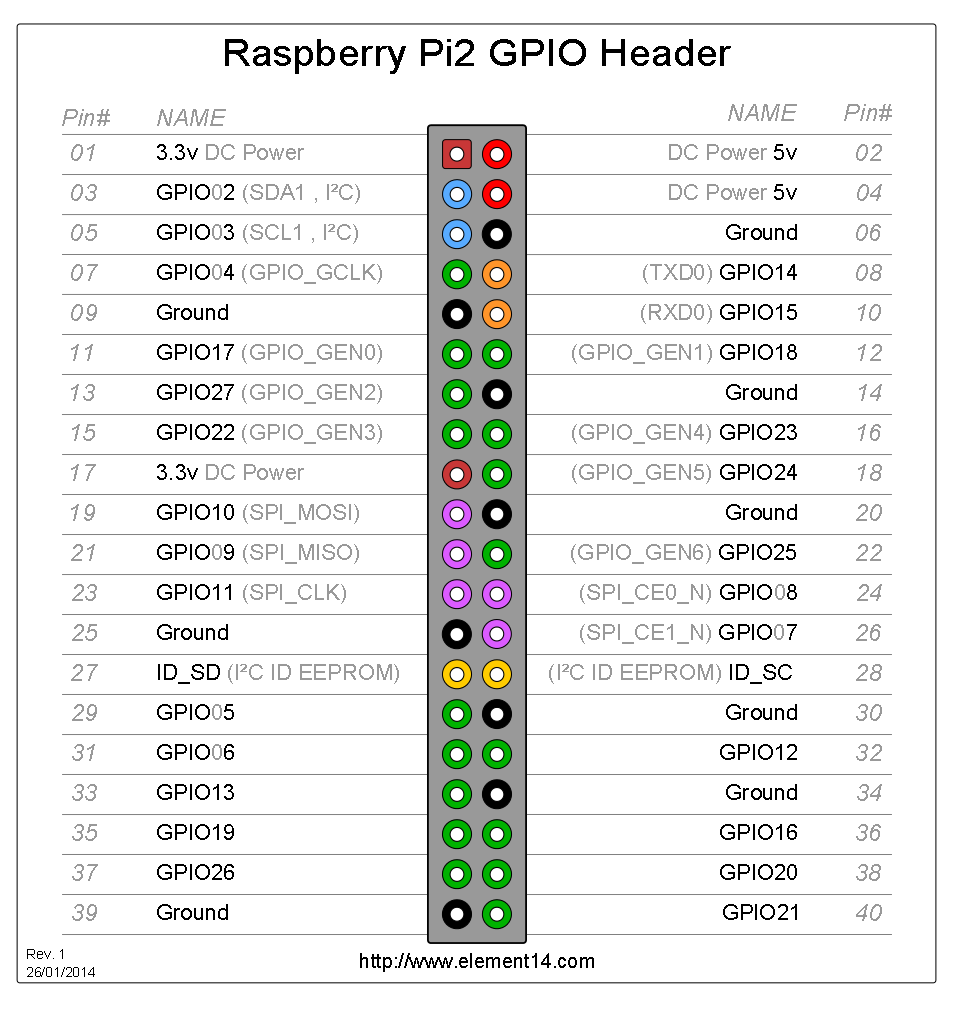
\includegraphics[scale=.4]{images/GPIO_Pi2.png}
	\caption{The pinout of the Raspberry Pi 2 model B, revision 2}
	\label{fig:gpioraspbi2}
\end{figure}

During the initial stages of using ROS we attempted to get the installation up and running on the Raspbian operating system (that is made for the Raspberry Pi). Raspbian is a modified version of the Debian distribution. The installation was done using the guide on the official Raspberry Pi website.\cite{raspiinstall}

After the installation, we installed the Indigo distribution of ROS, using their step-by-step guide for Raspbian.\cite{indigoins}
A source installation had to be done, due to poor support for the Raspbian OS, and this resulted in an 4-8 hour setup, due to the need for compiling, build and testing of the whole system. During the gathering of the different necessary packages needed for ROS, some unforeseen issues were encountered. Specifically the GMapping package caused some issues, since it required Python 2.7.1 and upwards. Even though a python version fitting the requirement was installed by default on the Raspbian, the GMapping package would not recognize it. Through troubleshooting it was then discovered that GMapping was looking for Python-2.7.1-ubuntu, instead of the Python-2.7.1-debian that was installed together with the Raspbian operating system.

Instead of continuing to deal with the ROS issues on the Raspbian installation, Ubuntu ARM was instead installed on the Raspberry Pi.\cite{ubuntuins}
The installation process using Ubuntu ARM was much faster and more fluent compared to installing ROS on the Raspbian installation, due to the much broader support for the Ubuntu OS. The installation only took couple of hours, by using the built-in package manager and because no installation was required from source.\cite{ubuntuROS}

